%-----------------------------------------------------------------
%	BASIC DOCUMENT LAYOUT
%-----------------------------------------------------------------
\documentclass[paper=a4, fontsize=12pt, twoside=semi, abstracton, listof=totoc, toc=left]{scrartcl}
\usepackage[T1]{fontenc}
\usepackage[utf8]{inputenc}
\usepackage{lmodern}
\usepackage{slantsc}
\usepackage{microtype}
\usepackage{mathtools} 
\usepackage[english]{babel}

% \usepackage[backend=bibtex, style=phys, sorting=none, citestyle=authoryear, maxbibnames=3, maxcitenames=2]{biblatex}
\usepackage[backend=bibtex, style=trad-abbrv, sorting=none, maxbibnames=3, maxcitenames=2]{biblatex}
\addbibresource{bibliography}
% \bibliographystyle{apalike}
\makeatletter
	\def\blx@maxline{77}
\makeatother

% Sectioning layout
\addtokomafont{sectioning}{\normalfont\bfseries}
\usepackage{tocstyle}
\usetocstyle{standard}
\renewcommand*\descriptionlabel[1]{\hspace\labelsep\normalfont\bfseries{#1}}
\usepackage[titletoc]{appendix}

% Empty pages
\usepackage{etoolbox}
\pretocmd{\toc}{\cleardoubleevenemptypage}{}{}
\pretocmd{\section}{\cleardoubleevenemptypage}{}{}
\pretocmd{\part}{\cleardoubleevenemptypage\thispagestyle{empty}}{}{}
\renewcommand\partheadstartvskip{\clearpage\null\vfil}
\renewcommand\partheadmidvskip{\par\nobreak\vskip 20pt\thispagestyle{empty}}

% Paragraph indentation behaviour
\setlength{\parindent}{0pt}
\setlength{\parskip}{0.3\baselineskip plus2pt minus2pt}
\newcommand{\sk}{\medskip\noindent}

% Fancy header and footer
\usepackage{fancyhdr}
\pagestyle{fancyplain}
\fancyhead[LO]{\thepage}
\fancyhead[CO]{}
\fancyhead[RO]{\nouppercase{\mytitle}}
\fancyhead[LE]{\nouppercase{\rightmark}}
% \fancyhead[LE]{\nouppercase{\leftmark}}
\fancyhead[CE]{}
\fancyhead[RE]{\thepage}
\fancyfoot{}
\renewcommand{\headrulewidth}{0.3pt}
\renewcommand{\footrulewidth}{0pt}
\setlength{\headheight}{13.6pt}

%-----------------------------------------------------------------
%	MATHS AND SCIENCE
%-----------------------------------------------------------------
\usepackage{amsmath,amsfonts,amsthm,amssymb}
\usepackage{xfrac}
\usepackage[a]{esvect}
\usepackage{chemformula}
\usepackage{graphicx}
	\graphicspath{{images/}}

\usepackage[arrowdel]{physics}
	\renewcommand{\vnabla}{\vec{\nabla}}
	% \renewcommand{\vectorbold}[1]{\boldsymbol{#1}}
	% \renewcommand{\vectorarrow}[1]{\vec{\boldsymbol{#1}}}
	% \renewcommand{\vectorunit}[1]{\hat{\boldsymbol{#1}}}
	\renewcommand{\vectorarrow}[1]{\vec{#1}}
	\renewcommand{\vectorunit}[1]{\hat{#1}}
	\renewcommand*{\grad}[1]{\vnabla #1}
	\renewcommand*{\div}[1]{\vnabla \vdot \va{#1}}
	\renewcommand*{\curl}[1]{\vnabla \cp \va{#1}}
	\let\rot\curl

% SI units
\usepackage[separate-uncertainty=true]{siunitx}
% \sisetup{range-phrase = \text{--}, range-units = brackets}
\sisetup{range-phrase = \text{--}, range-units = single}
\DeclareSIPrePower\quartic{4}
	%\DeclareSIUnit\micron{\micro\metre}

% Smaller trig functions
\newcommand{\Sin}{\trigbraces{\operatorname{s}}}
\newcommand{\Cos}{\trigbraces{\operatorname{c}}}
\newcommand{\Tan}{\trigbraces{\operatorname{t}}}

% Operator-style notation for matrices
\newcommand*{\mat}[1]{\hat{#1}}

% Matrices in (A|B) form via [c|c] option
\makeatletter
\renewcommand*\env@matrix[1][*\c@MaxMatrixCols c]{%
  \hskip -\arraycolsep
  \let\@ifnextchar\new@ifnextchar
  \array{#1}}
\makeatother

% Shorter \mathcal and \mathbb
\newcommand*{\mc}[1]{\mathcal{#1}}
\newcommand*{\mbb}[1]{\mathbb{#1}}

% Shorter ^\ast and ^\dagger
\newcommand*{\sast}{^{\star}{}}
\newcommand*{\sdag}{^{\dagger}{}}

% Blackboard bold identity
\usepackage{bbm}
\newcommand*{\bbid}{\mathbbm{1}}

% Shorter displaystyle
\newcommand*{\dsp}{\displaystyle}

% Inexact differential
\newcommand{\dbar}{\mathchar'26\mkern-12mu\mathrm{d}}
\newcommand{\indd}[1]{\dbar{#1}}

% Arrows with text and cancels for developments
\newcommand{\tikzmark}[1]{\tikz[overlay,remember picture] \node (#1) {};}
\tikzset{square arrow/.style={to path={-- ++(0,-.25) -| (\tikztotarget)}}}
\usepackage{cancel}

\newcommand*\acr[1]{\textscale{.85}{#1}}

%-----------------------------------------------------------------
%	OTHER PACKAGES
%-----------------------------------------------------------------
\usepackage{environ}

%Left numbered equations
\makeatletter
	\NewEnviron{Lalign}{\tagsleft@true\begin{align}\BODY\end{align}}
\makeatother

% Plots and graphics
\usepackage{pgfplots}
\usepackage{tikz}
\usepackage{color}
	\makeatletter
		\color{black}
		\let\default@color\current@color
	\makeatother

% Richer enumerate, figure, and table support
\usepackage{enumerate}
\usepackage[shortlabels]{enumitem}
\usepackage{float}
\usepackage{tabularx}
\usepackage{booktabs}
	%\setlength{\intextsep}{8pt}
% \numberwithin{equation}{section}
% \numberwithin{figure}{section}
% \numberwithin{table}{section}
% \counterwithin{lstlisting}{section}

% No indentation after certain environments
\makeatletter
\newcommand*\NoIndentAfterEnv[1]{%
	\AfterEndEnvironment{#1}{\par\@afterindentfalse\@afterheading}}
\makeatother
%\NoIndentAfterEnv{thm}
\NoIndentAfterEnv{defi}
\NoIndentAfterEnv{example}
\NoIndentAfterEnv{table}

% Misc packages
\usepackage{todonotes}
%\usepackage{array}
%\usepackage{multirow}

% Print DOI only if there's no URL
\renewbibmacro*{doi+eprint+url}{%
  \iftoggle{bbx:doi}
    {\iffieldundef{url}{\printfield{doi}}{}}
    {}%
  \newunit\newblock
  \iftoggle{bbx:eprint}
    {\usebibmacro{eprint}}
    {}%
  \newunit\newblock
  \iftoggle{bbx:url}
    {\usebibmacro{url+urldate}}
    {}}

%-----------------------------------------------------------------
%	SYNTAX HIGHLIGHTING
%-----------------------------------------------------------------
\usepackage[formats]{listings}
\usepackage{relsize}
\usepackage{chngcntr}

\renewcommand{\lstlistingname}{Snippet}
\renewcommand{\lstlistlistingname}{List of snippets}

\lstloadlanguages{c,R,awk,bash}
% \lstdefinelanguage{Renhanced}[]{R}{%
% 	morekeywords={acf,ar,arima,arima.sim,colMeans,colSums,is.na,is.null,%
% 	mapply,ms,na.rm,nlmin,replicate,row.names,rowMeans,rowSums,seasonal,%
% 	sys.time,system.time,ts.plot,which.max,which.min,%
% 	rename,mutate,unite,select,filter,left_join,group_by,dplyr::select,%
% 	ggplot,aes,geom_line,geom_hline,geom_point,geom_path,geom_errorbar,%
% 	geom_abline,geom_smooth%
% 	geom_cartogram,coord_proj,scale_x_longitude, scale_y_latitude,%
% 	labs,guides,annotate,theme,rowwise,%
% 	scale_linetype_manual,scale_colour_manual,scale_x_log10,scale_y_log10,%
% 	attr,paste,paste0,bind_rows,str_trim,as.numeric,as.dataframe,data.frame},
% 	deletekeywords={c,range,step},
% 	alsoletter={.,_,::},
% 	otherkeywords = {!,!=,~,\$,*,\&,\%/\%,\%*\%,\%\%,\%>\%,<-,<<-,\% in \%}
% 	}

\newcommand*{\inline}{\lstinline[basicstyle=\normalsize\ttfamily]}


\lstset{language=c,
		frame=tb,
		% captionpos=b,
		tabsize=2,
		% showtabs=true,
		breaklines=true,
		breakatwhitespace=true,
		basicstyle=\smaller\ttfamily,
		numbers=left,
		numberstyle=\tiny,
		numbersep=7.5pt,
		% commentstyle=\textsl,
		xleftmargin=3ex}
\lstset{escapeinside={(*}{*)}}   % for (*\ref{ }*) inside lstlistings (Scode)

\lstdefinestyle{output}{
	language=,
	% showtabs=true,
	% showspaces=true,
	numbers=none,
	frame=tblr,
	% columns=fullflexible,
	% backgroundcolor=\color{blue!10},
	numbers=none,
	xleftmargin=3ex}

% Inline listing inside maths environments
\expandafter\patchcmd\csname \string\lstinline\endcsname{%
	\leavevmode
	\bgroup
}{%
	\leavevmode
	\ifmmode\hbox\fi
	\bgroup
}{}{%
	\typeout{Patching of \string\lstinline\space failed!}%
}

\lstnewenvironment{algorithm}[1][]
{
    \renewcommand\lstlistingname{Algorithm}
    \lstset{language=c,
		frame=tb,
		% captionpos=b,
		tabsize=2,
		% showtabs=true,
		breaklines=true,
		breakatwhitespace=true,
		basicstyle=\smaller\ttfamily,
		numbers=left,
		numberstyle=\tiny,
		numbersep=7.5pt,
		% commentstyle=\textsl,
		xleftmargin=3ex,
        #1}
}{}

\lstnewenvironment{script}[1][]
{
    \renewcommand\lstlistingname{Script}
    \lstset{language=c,
		frame=tb,
		% captionpos=b,
		tabsize=2,
		% showtabs=true,
		breaklines=true,
		breakatwhitespace=true,
		basicstyle=\smaller\ttfamily,
		numbers=left,
		numberstyle=\tiny,
		numbersep=7.5pt,
		% commentstyle=\textsl,
		xleftmargin=3ex,
        #1}
}{}

%-----------------------------------------------------------------
%	THEOREMS
%-----------------------------------------------------------------
\usepackage{thmtools}

% Theroems layout
\declaretheoremstyle[
	spaceabove=6pt, spacebelow=6pt,
	headfont=\normalfont,
	notefont=\mdseries, notebraces={(}{)},
	bodyfont=\small,
	postheadspace=1em,
]{small}

\declaretheorem[style=plain,name=Theorem,qed=$\square$,numberwithin=section]{thm}
\declaretheorem[style=plain,name=Corollary,qed=$\square$,sibling=thm]{cor}
\declaretheorem[style=plain,name=Lemma,qed=$\square$,sibling=thm]{lem}
\declaretheorem[style=definition,name=Definition,qed=$\blacksquare$,numberwithin=section]{defi}
\declaretheorem[style=definition,name=Example,qed=$\blacktriangle$,numberwithin=section]{example}
\declaretheorem[style=small,name=Proof,numbered=no,qed=$\square$]{sproof}

%-----------------------------------------------------------------
%	DEDICATION ENVIRONMENT
%-----------------------------------------------------------------

\newenvironment{mydedication}
	{\clearpage           % we want a new page
	\thispagestyle{empty}% no header and footer
	\vspace*{\stretch{1}}% some space at the top
	\itshape             % the text is in italics
	\raggedleft          % flush to the right margin
	}
	{\par % end the paragraph
	\vspace{\stretch{3}} % space at bottom is three times that at the top
	\clearpage           % finish off the page
	}

%-----------------------------------------------------------------
%	PDF INFO AND HYPERREF
%-----------------------------------------------------------------
\usepackage{hyperref}
\hypersetup{colorlinks, citecolor=black, filecolor=black, linkcolor=black, urlcolor=black}
\usepackage{cleveref}
	\crefname{section}{\S}{\SS}
	\Crefname{section}{\S}{\SS}
	\crefname{listing}{snippet}{}

\newcommand*{\mytitle}{The A* Algorithm}
\newcommand*{\mysubtitle}{An Implementation Using C}
\newcommand*{\myauthor}{Alfredo Hernández \and Ruth Kristianingsih}
\newcommand*{\myuni}{Universitat Autònoma de Barcelona}
\newcommand*{\mydate}{10th February 2018}

\pdfstringdefDisableCommands{\def\and{and }}

\usepackage{hyperxmp}
\hypersetup{pdfauthor={\myauthor}, pdftitle={\mytitle: \mysubtitle}}

%-----------------------------------------------------------------
%	TITLE SECTION AND DOCUMENT BEGINNING
%-----------------------------------------------------------------
\newcommand{\horrule}[1]{\rule{\linewidth}{#1}}
\title{
	\normalfont
% 	\small \scshape{\myuni} \\ [25pt]
    
\includegraphics[width=0.5\textwidth]{images/uab-logo} \\
	\horrule{0.5pt} \\ [0.4cm]
	\huge \scshape{\mytitle} \\
	\Large \scshape{\mysubtitle} \\
	\horrule{2pt} \\ [0.5cm]
}
\author{\myauthor }
% \\ \footnotesize Supervised by: \mysupervisor \\ \footnotesize Academic tutor: \mytutor}
\date{\mydate}

\begin{document}

\clearpage\maketitle
\thispagestyle{empty}
\addtocounter{page}{-1}

%-----------------------------------------------------------------
%	DEDICATION
%-----------------------------------------------------------------
% \begin{mydedication}
% 	Dedicated to RMT, Val \& the Brotherhood
% \end{mydedication}

%-----------------------------------------------------------------
%	DOCUMENT BODY
%-----------------------------------------------------------------
% \cleardoubleevenemptypage
% %-----------------------------------------------------------------
%	ABSTRACT
%	!TEX root = ./../main.tex
%-----------------------------------------------------------------
\cleardoubleevenemptypage
\thispagestyle{empty}
\phantomsection
\addcontentsline{toc}{section}{Abstract}
\begin{abstract}
	Crime Data Analysis is an already established yet flourishing topic in the United States. Despite that, there is no public user-friendly global data hub to visualise crime statistics across the US territory. The goal of this work is to create dynamic time series visualisations of the evolution of crime in different cities of the US. The mission of this work is to develop visualisation tools in order to further ease the access to already open data. Using the R language we gather open databases of different cities and unify the data into a single standard format, leading to straightforward comparative methods. We would like to see whether or not crime statistics change significantly throughout the different regions of the US and if there are clear trends that help us identify geographical differences in the American society. Last but not least, we would like to look for temporal patterns that could be identified with major global or local events.
\end{abstract}


\pdfbookmark[1]{\contentsname}{toc}
\tableofcontents

%-----------------------------------------------------------------
%	INTRODUCTION
%	!TEX root = ./../main.tex
%-----------------------------------------------------------------
\section{Introduction}

The knapsack problem is a classic and widely studied computational problem in combinatorial optimization. Given a set of items, each with a weight and a value, determine the number of each item to include in a collection so that the total weight is less than or equal to a given limit and the total value is as large as possible. It derives its name from the problem faced by someone who is constrained by a fixed-size knapsack and must fill it with the most valuable items. Because the knapsack problem is a very general problem in combinatorial optimization, it has applications in almost every field. For instance, in economics, the knapsack problem
is analogous to a simple consumption model given a budget constraint. In other words, we choose from a
list of objects to buy, each with a certain utility, subject to the budget constraint. One of the most interesting applications is in solving truck loading problem. We have to load a truck with some goods. The values and the weights of these goods are listed here\footnote{\url{http://mat.uab.cat/~alseda/MasterOpt/KnapsackData.dat}}, and the truck can carry a maximum weight of 600 Kg. We want to maximize the total value of the taken goods.

\begin{table}[H]
\centering
% \resizebox{\textwidth}{!}{%
    \begin{tabular}{cc}
        \toprule
        \toprule
        values & weights \\
        \midrule
        18     & 17      \\
        11     & 20      \\
        15     & 15      \\
        18     & 12      \\
        15     & 13      \\
        7      & 20      \\
        17     & 13      \\
        15     & 13      \\
        22     & 16      \\
        16     & 15      \\
        18     & 14      \\
        10     & 15      \\
        13     & 21      \\
        15     & 13      \\
        16     & 20      \\
        15     & 19      \\
        12     & 7       \\
                \bottomrule
    \end{tabular}
    \hspace{5pt}
    \begin{tabular}{cc}
        \toprule
        \toprule
        values & weights \\
        \midrule
        13     & 11      \\
        12     & 16      \\
        11     & 12      \\
        14     & 14      \\
        17     & 17      \\
        12     & 18      \\
        15     & 16      \\
        7      & 17      \\
        16     & 25      \\
        16     & 27      \\
        12     & 15      \\
        16     & 7       \\
        13     & 18      \\
        16     & 13      \\
        12     & 13      \\
        10     & 24      \\
        11     & 18      \\
        \bottomrule
    \end{tabular}
    \hspace{5pt}
    \begin{tabular}{cc}
        \toprule
        \toprule
        values & weights \\
        \midrule
        13     & 17      \\
        15     & 11      \\
        16     & 18      \\
        15     & 13      \\
        11     & 16      \\
        14     & 14      \\
        21     & 16      \\
        11     & 21      \\
        13     & 17      \\
        10     & 14      \\
        14     & 18      \\
        18     & 16      \\
        17     & 15      \\
        14     & 11      \\
        11     & 23      \\
        15     & 19      \\
        --     & --      \\
        \bottomrule
    \end{tabular}
    \caption{Values and Weights of Goods to Optimize}
    \label{tab:problemdata}
\end{table}
%-----------------------------------------------------------------
%	THEORITICAL BACKGROUND
%	!TEX root = ./../main.tex
%-----------------------------------------------------------------
\section{Theoretical Background}

%-----------------------------------------------------------------
\subsection{Knapsack Problem}
The knapsack problem is a classical 0--1 combinatorial optimization problem that can be applied to various fields such as economics. A set of $n$ items, each item $i (i = 1, \dots , n)$ has assigned a value (for instance price) $v_i$ and an item weight value $w_i$ for each item $i (i = 1, \dots , n)$. The problem is to identify a subset of all items that leads to the highest total profit and does not exceed the resource upper bound $W$ . Then, the knapsack can be formulated as:

\begin{align}\label{eq:maxf}
    \text{maximize }  f = \sum_{i=1}^{n} v_i x_i, \text{ where } x_i = 
    \begin{cases}
        1 & \text{if the item is in the bag} \\
        0 & \text{otherwise}
    \end{cases}
\end{align}

subject to the constraints
\begin{align}\label{eq:cons}
    \sum_{i=1}^{n} w_i x_i \leq W 
    \qc x_i \in \qty{0,1}
\end{align}

The variable $x_i$ is an indicator of item $i$. If $x_i$ is set to \num{1}, it means item $i$ is selected, or \num{0} means item $i$ is not selected for $i = 1, \dots , n$. \eqref{eq:maxf} represents the total value or profit of selection items and \eqref{eq:cons} constraint.

%-----------------------------------------------------------------
\subsection{Simulated Annealing}\label{sec:sa}
Simulated annealing is so named because of its analogy to the process of physical annealing with solids, in which a crystalline solid is heated and then allowed to cool very slowly until it achieves its most regular possible crystal lattice configuration (i.e., its minimum lattice energy state), and thus is free of crystal defects. If the cooling schedule is sufficiently slow, the final configuration results in a solid with such superior structural integrity. Simulated annealing establishes the connection between this type of thermodynamic behavior and the search for global minimum for a discrete optimization problem. Furthermore, it provides an algorithmic means for exploiting such a connection.

At each iteration of a simulated annealing algorithm applied to a discrete optimization problem, the objective function generates values for two solutions (the current solution and a newly selected solution) are compared. Improving solutions are always accepted, while a fraction of non-improving (inferior) solutions are accepted in the hope of escaping local optima in search of global optima. The probability of accepting non-improving solutions depends on a temperature parameter, which is typically non-increasing with each iteration of the algorithm.

\subsubsection*{Steps of the Algorithm}
The usual steps for Simulated Annealing are presented below:
\begin{enumerate}[(i)]
    \item \emph{Initialize}: start with a random initial placement. Initialize a very high “temperature”.
    \item \emph{Move}: perturb the placement through a defined move.\label{step2}
    \item \emph{Calculate Score}: Calculate the change in the score due to the move made. 
    \item \emph{Choose}: depending on the change in score, accept or reject the move, where probability of acceptance depends on the current “temperature”. For this point we will use the Classical Metropolis Method.
    \item \emph{Update and Repeat}: update the temperature value by
    lowering the temperature following a cooling schedule. Go back to \ref{step2}.
\end{enumerate}

The process is done when the “Freezing Point” is reached.

\subsubsection*{Acceptance Rule}
In thermodynamical systems, it is usual to use the Classical Metropolis Method to compute the probability of changing from one state to another~\cite{Frenkel2002}. In simple words, the method consists on doing a random change in the system and accept the change in accordance to the following acceptance rule:
\begin{align}
	\acc{\va{x}}{\va{y}} =
	\begin{cases}
		e^{- \beta \qty[H(\va{y}) - H(\va{x})]} & H(\va{y}) > H(\va{x}) \\
		1                                       & H(\va{y}) < H(\va{x})
	\end{cases}
\end{align}
where $H(\va{x})$ is the energy of the state $\va{x}$, $\beta = 1/(k_{B} T)$, and $T$ is the temperature.

Notice that this has the same physical interpretation we would expect in a thermodynamical system:
\begin{itemize}
	\item Limit $T \to 0$ ($\beta \to \infty$): the system only accepts changes that minimize the energy:
	\begin{align*}
		\acc{\va{x}}{\va{y}} =
		\begin{cases}
			0 & H(\va{y}) > H(\va{x}) \\
			1 & H(\va{y}) < H(\va{x})
		\end{cases}
	\end{align*}
	\item Límit $T \to \infty$ ($\beta \to 0$): the system accepts all changes, which maximizes the entropy.
\end{itemize}

In our problem, the \emph{energy} can be interpreted as follows:
\begin{align}
    H(\va{x}) = \displaystyle \sum_{i=1}^{n} v_i x_i
\end{align}

\subsubsection*{Cooling Schedule}
In the process of annealing a metal, if the heating temperature is sufficiently high to ensure random state and the cooling process is slow enough to ensure thermal equilibrium, then the atoms will place themselves in a pattern that corresponds to the global energy minimum of a perfect crystal.

For this reason, we need to choose very carefully our Cooling Schedule. We have decided to use a curve that decreases slowly the temperature until the particles arrange themselves in the ground state of the solid. We use the following formula:
\begin{align}
    T_{i} = \frac{T_{0} \cdot \tanh(- \ln(i) + 10) + 1 )}{2} 
\end{align}

The idea behind it is to let the algorithm quickly discard bad configurations in the very beginning (high temperature), and explore different configurations close to the optimal solution in the final steps (low temperatures). The plot of the our cooling schedule can be seen in \cref{fig:temp}.
\begin{figure}[H]
    \centering
    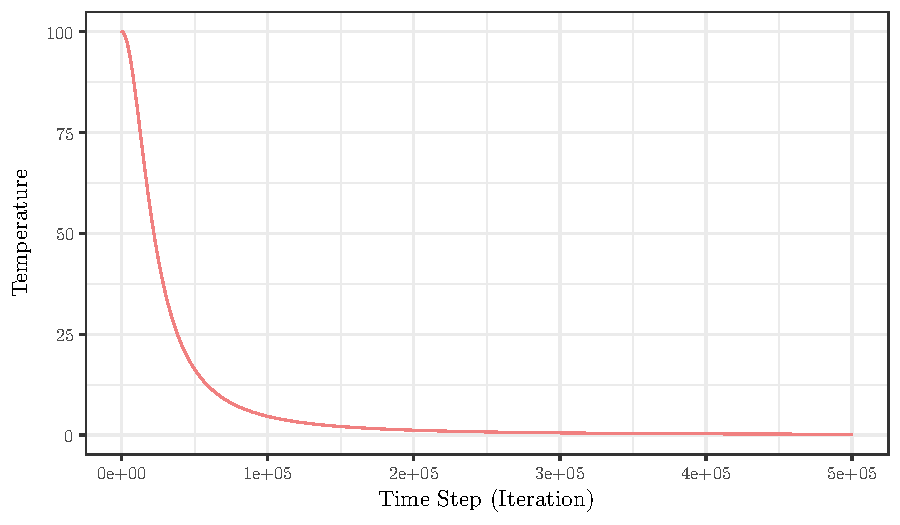
\includegraphics[width=\textwidth]{images/temp}
    \caption{Evolution of the Temperature Following a Cooling Schedule}
    \label{fig:temp}
\end{figure}










%-----------------------------------------------------------------
%	STATISTICAL ANALYSIS
%	!TEX root = ./../main.tex
%-----------------------------------------------------------------
\section{Implementation of the Program}\label{sec:implementation}

\subsection{Preprocessing the Data}
Since the data provided includes a header, we decided the get rid of it using AWK, and change the format to store it in a \inline{.csv} file:
\begin{lstlisting}[language=awk]
BEGIN{
	FS = " "
	OFS = ","
}
NR > 1 && NF == 2 {
	print $1, $2
}
\end{lstlisting}

We just run it as usual:
\begin{lstlisting}[language=bash]
awk -f clean_data.awk KnapsackData.dat > data.csv
\end{lstlisting}


\subsection{Algorithm in Python}
The algorithm in Python 3.5 is programmed mainly using the NumPy library. 

First of all, we use Pandas to read and process the file with the data:
\begin{lstlisting}
data = pd.read_csv('data.dat')
values = np.array(data["values"])
weights = np.array(data["weights"])
num_items = len(data)
\end{lstlisting}


Two important parameters in the algorithm are the total weight and the total value of the items in the truck. For this reason, we have defined the \inline{get_weight()} and \inline{ get_value()} functions:
\begin{lstlisting}
def get_weight(individual, weights):
	return int(np.sum(individual * weights))
\end{lstlisting}

\begin{lstlisting}
def get_value(individual, values, weights):
	total_weight = get_weight(individual, weights)
	if (total_weight <= 600):
		total_value = np.sum(individual * values)
	else:
		total_value = - pow(total_weight, 100)
	return int(total_value)
\end{lstlisting}

Where the \inline{individual} is the array $\va{x}$ array of zeroes and ones used as an indicator of the present items in the truck.


We use a simple Monte Carlo method to mutate the elements $x_{i}$ of the individual:
\begin{lstlisting}
def random_bool():
	return np.random.randint(2)
\end{lstlisting}


For the Simulated Annealing we define a function which is just a fully fledged version of the algorithm we described in \cref{sec:sa}:
\begin{lstlisting}
def simulated_annealing(individual, MAX_ITER):
	for iter in range(0, MAX_ITER):
		# Temperature cooling schedule
		temp[iter] = MAX_TEMP * 0.5 * (tanh(-log(iter+1) + 10) + 1 )

		# Exploring the neighbourhood
		individual_new = np.copy(individual)
		for m in range(0, 5):
			index = np.random.randint(num_items)
			individual_new[index] = random_bool()

		# Total value of items inside the truck
		value_old = get_value(individual, values, weights)
		value_new = get_value(individual_new, values, weights)

		# Acceptance probabilities
		if (value_old < value_new):
			prob[iter] = 1
		else:
			prob[iter] = exp(-(value_old - value_new) / temp[iter])

		# Acceptance rule
		if (float(np.random.random(1)) < prob[iter]):
			individual = np.copy(individual_new)

		# Update total value and weight
		sol_values[iter] = get_value(individual, values, weights)
		sol_weights[iter] = get_weight(individual, weights)
	return individual
\end{lstlisting}

To run the algorithm, and store the final solution we just call the function we defined above:
\begin{lstlisting}
solution = simulated_annealing(individual, MAX_ITER)
\end{lstlisting}

\bigskip
To run the algorithm, we just need to run the following:
\begin{lstlisting}
python knapsack_sa.py
\end{lstlisting}
% \include{./contents/4-results}
%-----------------------------------------------------------------
%	CONCLUSIONS
%	!TEX root = ./../main.tex
%-----------------------------------------------------------------
\section{Results and Discussion}\label{sec:res}

Results of the preceding implementation in \Cref{sec:implementation} will be presented in this section. Mainly, the objective of this analysis is finding optimal path from Barcelona to Sevilla. In \cref{fig:bcntosevilla}, it is shown the map of optimal path computed with the distance \SI{958815.01}{\m} with a number of optimal nodes of \num{6649} as seen in \cref{tab:results}. As a performance indicator, we used \inline{perf stat}; the program took around \SI{11.972}{\s} to obtain and print the optimal path to a \inline{solution.csv} file. 
\begin{figure}[H]
    \centering
    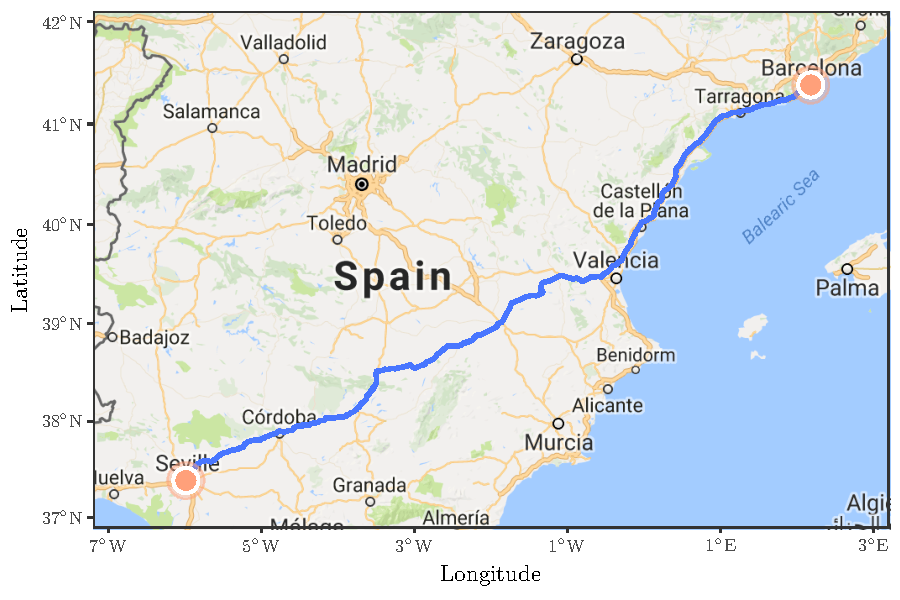
\includegraphics[width=0.9\textwidth]{images/solution}
    \caption{Optimal Path from Barcelona to Sevilla}
    \label{fig:bcntosevilla}
\end{figure}

\begin{table}[H]
  \centering
  \begin{tabular}{l c}
      \toprule
      \toprule
      Creating the binary file                  & \SI{28.817}{\s} \\
      Creating the binary file (\texttt{Ofast}) & \SI{28.732}{\s} \\
      Finding the optimal path                  & \SI{11.972}{\s} \\
      Finding the optimal path (\texttt{Ofast}) & \SI{8.599}{\s}  \\
      \midrule
      Optimal path distance    & \SI{958815.01}{\m} \\
      Number of nodes          & \num{6649} \\
      \bottomrule
  \end{tabular}
  \caption{Information about the Performance and Results of Implemented Program}
  \label{tab:results}
\end{table}

In case one wanted to apply the A* Algorithm to two arbitrary nodes in Spain, we have implemented another version of the main program (\inline{a-star-input.c}) that allows the user to select the start and goal nodes\footnote{One can easily find node IDs using \url{https://nominatim.openstreetmap.org}, or grepping the \texttt{.csv} database}. 

To test this interactive version of the program, we tried to find the optimal path in smaller area using the implemented algorithm from Barcelona (node \inline{240949599}) to UAB (node \inline{255403621}):
\begin{lstlisting}[language=bash]
gcc -lm -Ofast functions.c a-star-input.c -o astar-input
./astar-input 240949599 255403621
\end{lstlisting}

The optimal path computed is illustrated in \cref{fig:bcntouab}. The distance is around \SI{19839.10}{\m} with the number of nodes is \num{331}, and the program need about \SI{0.916}{\s} to get the results as summarized in \cref{tab:results-uab}.

\begin{figure}[H]
    \centering
    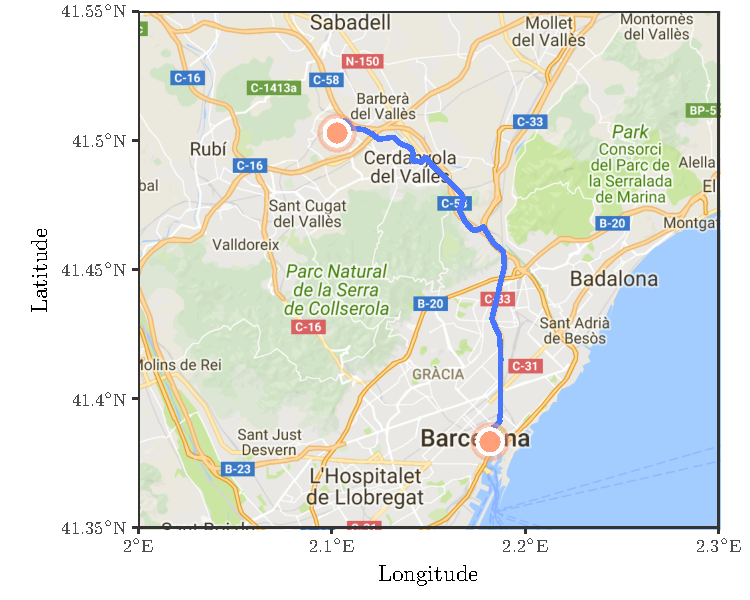
\includegraphics[width=0.8\textwidth]{images/solution-uab}
    \caption{Optimal Path from Barcelona to UAB}
    \label{fig:bcntouab}
\end{figure}


\begin{table}[H]
  \centering
  \begin{tabular}{l c}
      \toprule
      \toprule
      Finding the optimal path                  & \SI{0.916}{\s} \\
      Finding the optimal path (\texttt{Ofast}) & \SI{0.819}{\s} \\
      \midrule
      Optimal path distance    & \SI{19839.10}{\m} \\
      Number of nodes          & \num{331} \\
      \bottomrule
  \end{tabular}
  \caption{Information about the Performance and Results of Implemented Program}
  \label{tab:results-uab}
\end{table}

\newpage
\subsection{Further Improvements}

Some different experiments, for instance changing the heuristic functions have been left for the future work due to lack of time. There are some ideas that we would like to try during the implementation of A* algorithm. This analysis report mainly focused on finding path from Barcelona to Sevilla, leaving the finding optimal path from different places. For this reason, we propose some ideas to be tested and implemented as part of future work and further improvements as follows:
\begin{enumerate}[(i)]
	\item Try different heuristic functions and compare the performance of the algorithm.
    \item Include larger area to be tested to find optimal path, for instance whole area of Europe (we are not even sure the whole Spain area is included, as some of the nodes we tried to experiment with were not in the \inline{.csv} file).
    \item For the latter, we would like to define some of the variables in a less \emph{hardcoded} way, especially when dealing with sizes memory allocation.
    \item Trying to find an optimal path from Barcelona to Madrid the A* Algorithm got apparently stuck in a cyclic loop at some point. This is because a node in the \inline{CLOSED} list could end up back again in the \inline{OPEN} list. This is an issue that would be interesting to address.
	\item Improve the performance of the programs in terms of memory. Surely some variables could have been freed after not needing them anymore.
%     \item Implementing Jump Point Search (JPS) which is an optimization to the A* search algorithm for uniform-cost grids.
\end{enumerate}




%-----------------------------------------------------------------
%	BIBLIOGRAPHY
%-----------------------------------------------------------------

\nocite{Pearl1984}
\nocite{Sean2010}
\nocite{Erickson2014}

\printbibliography[heading=bibintoc]
% \setcounter{secnumdepth}{0}
% \section{References}
% \printbibliography[title={Articles}, type=article, heading=subbibliography]
% \printbibliography[title={Books}, type=book, heading=subbibliography]
% \printbibliography[title={Websites}, type=online , heading=subbibliography]
% \printbibliography[title={Basic}, keyword=basic , heading=subbibliography]

% \clearpage
% \begin{appendices}
% \pagenumbering{arabic}% resets `page` counter to 1
% \renewcommand*{\thepage}{A\arabic{page}}
% %-----------------------------------------------------------------
%	APPENDIX B
%	!TEX root = ./../main.tex
%-----------------------------------------------------------------
\section{Figures}\label{app:figures}
The figures shown in this appendix are figures that are referenced in and important for the main text that could not be included for lenght reasons.

\subsection*{Statistical Analysis}

\begin{figure}[H]
	\centering
	\includegraphics[width=\textwidth]{images/sstplot_each}
	\caption{Plot of Time Series of SST for Each Year}
	\label{fig:sstplot-each}
\end{figure}

\newpage

\begin{figure}[H]
	\centering
	\includegraphics[width=0.9\textwidth]{images/windplot_each}
	\caption{Plot of Time Series of Wind Speed for Each Year}
	\label{fig:windplot-each}
\end{figure}

%-----------------------------------------------------------------
\subsection*{Probability Distribution of the Data}

\begin{figure}[H]
	\centering
	\includegraphics[width=\textwidth]{images/ssthist_stable_each}
	\caption{Plot of Time Series of SST for Each Year}
	\label{fig:ssthist-each}
\end{figure}

\begin{figure}[H]
	\centering
	\includegraphics[width=\textwidth]{images/windhist_stable_each}
	\caption{Plot of Time Series of Wind Speed for Each Year}
	\label{fig:windhist-each}
\end{figure}

%-----------------------------------------------------------------
\subsection*{Measure of Dependence Analysis}

\begin{figure}[H]
	\centering
	\includegraphics[width=0.9\textwidth]{images/sstacf_each}
	\caption{Plot of ACF of SST for Each Year}
	\label{fig:sstacf-each}
\end{figure}

\begin{figure}[H]
	\centering
	\includegraphics[width=0.9\textwidth]{images/windacf_each}
	\caption{Plot of ACF of Wind Speed for Each Year}
	\label{fig:windacf-each}
\end{figure}

\begin{figure}[H]
	\centering
	\includegraphics[width=0.9\textwidth]{images/ccf_each}
	\caption{Plot of CCF of Wind Speed and SST for Each Year}
	\label{fig:windacf-each}
\end{figure}

%-----------------------------------------------------------------
\subsection*{Correlation in Frequency Domain}

% \begin{figure}[H]
% 	\centering
% 	\includegraphics[width=\textwidth]{images/periodo_nor_sst.jpeg}
% 	\caption{Plot of Periodogram in normal of SST for Each Year}
% 	\label{fig:peri_nor_sst_each}
% \end{figure}

\begin{figure}[H]
	\centering
	\includegraphics[width=0.9\textwidth]{images/sstper_each}
	\caption{Plot of Periodogram in Log Scale of SST for Each Year}
	\label{fig:peri_log_sst_each}
\end{figure}

% \begin{figure}[H]
% 	\centering
% 	\includegraphics[width=\textwidth]{images/periodo_nor_wind.jpeg}
% 	\caption{Plot of Periodogram in normal of Wind Speed for Each Year}
% 	\label{fig:peri_nor_wind_each}
% \end{figure}

\begin{figure}[H]
	\centering
	\includegraphics[width=0.9\textwidth]{images/windper_each}
	\caption{Plot of Periodogram in Log Scale of Wind Speed for Each Year}
	\label{fig:peri_log_wind_each}
\end{figure}
% %-----------------------------------------------------------------
%	APPENDIX A
%	!TEX root = ./../main.tex
%-----------------------------------------------------------------
\section{Developed code}\label{app:code}
\renewcommand{\lstlistingname}{Script}

\lstinputlisting[firstline = 1, label = scr:stat,%
	caption = \inline{statistical-analysis.R} - Code Used for the Statistical Analysis  ]%
	{code/statistical-analysis.R}

\lstinputlisting[firstline = 1, label = scr:fits,%
	caption = \inline{find-fits.R} - Code Used to Find the Fit Models for SST and Wind Speed ]%
	{code/find-fits.R}
	
\lstinputlisting[firstline = 1, label = scr:acf-ccf,%
	caption = \inline{acf-ccf-ts-functions.R} - Code Used to Find the ACF and CCF Functions ]%
	{code/acf-ccf-ts-functions.R}
	
\lstinputlisting[firstline = 1, label = scr:peri,%
	caption = \inline{periodogram.R} - Code Used to Find Correlations in the Frequency Domain ]%
	{code/periodogram_ggplot.R}
% \end{appendices}

\end{document}
